\documentclass[aspectratio=169, 11pt]{beamer}

% Packages
\usepackage[utf8]{inputenc}
\usepackage{amsmath, amssymb, amsfonts}
\usepackage{graphicx}
\usepackage{booktabs}
\usepackage{ragged2e}
\usepackage{minted}
\usepackage{xcolor}
\usepackage{tikz}
\usepackage{algorithm}
\usepackage{algorithmic}
\usepackage{listings}
\usepackage{tcolorbox}

\usetikzlibrary{arrows.meta,positioning,fit,shapes.symbols}
\usetikzlibrary{arrows,shapes}
\definecolor{LightGray}{gray}{0.975}
\definecolor{links}{HTML}{2A1B81}
\hypersetup{colorlinks,linkcolor=,urlcolor=blue}
\AtBeginEnvironment{minted}{%
    \renewcommand{\fcolorbox}[4][]{#4}
}

\title[Tree-Based Methods]{ML101 \\ Chapter 08: Tree-Based Methods}
\subtitle{An Introduction to Statistical Learning, ISLRv2}
\author{James, Witten, Hastie \& Tibshirani}
\date{\today}

% Remove navigation symbols
\setbeamertemplate{navigation symbols}{}

\defbeamertemplate*{footline}{shadow theme}{
    \leavevmode
    \hbox{
        \begin{beamercolorbox}[
                wd =        0.33\paperwidth,
                ht =        2.5ex,
                dp =        1.125ex,
                leftskip =  0.3cm plus1fil,
                rightskip = 0.3cm
            ]{author in head/foot}
            \flushleft ML101
        \end{beamercolorbox}
        \begin{beamercolorbox}[
                wd =        0.33\paperwidth,
                ht =        2.5ex,
                dp =        1.125ex,
                leftskip =  0.3cm plus1fil,
                rightskip = 0.3cm
            ]{author in head/foot}
            \insertshorttitle
        \end{beamercolorbox}
        \begin{beamercolorbox}[
                wd =        0.33\paperwidth,
                ht =        2.5ex,
                dp =        1.125ex,
                leftskip =  0.3cm plus1fil,
                rightskip = 0.3cm
            ]{title in head/foot}
            \hfill \insertframenumber\,/\,\inserttotalframenumber%
        \end{beamercolorbox}
    }
}

\AtBeginSection[]
{
     \begin{frame}<beamer>
     \frametitle{Plan}
     \tableofcontents[currentsection]
     \end{frame}
}

\usefonttheme{serif}

\newcommand\Wider[2][18mm]{%
    \makebox[\linewidth][c]{%
        \begin{minipage}{\dimexpr\textwidth+#1\relax}
            \raggedright#2
        \end{minipage}%
    }%
}
\newcommand\userinput[1]{\textbf{#1}}

\begin{document}

\frame{\titlepage}

\begin{frame}{An Introduction to Statistical Learning with Applications in R}{a.k.a. ISLR}
    \centering
    
\includegraphics[height=0.7\textheight]{figures/book_cover} \\
    \vspace{4mm}
    {
        \tiny
        Content has been extracted from \textit{An Introduction to Statistical Learning with Applications in R}, Second Edition, by James, Witten, Hastie \& Tibshirani. Springer. 2023.\\
        Visit \url{https://www.statlearning.com/}.\\
    }
\end{frame}

\begin{frame}{Tree-based Methods}
    \begin{itemize}
        \item Here we describe \textbf{tree-based} methods for regression and classification.
        \item These involve \textbf{stratifying} or \textbf{segmenting} the predictor space into a number of simple regions.
        \item Since the set of splitting rules used to segment the predictor space can be summarized in a tree, these types of approaches are known as \textbf{decision-tree} methods.
    \end{itemize}
\end{frame}

\begin{frame}{Pros and Cons}
    \begin{itemize}
        \item Tree-based methods are simple and useful for interpretation.
        \item However they typically are not competitive with the best supervised learning approaches in terms of prediction accuracy.
        \item Hence we also discuss \textbf{bagging}, \textbf{random forests}, and \textbf{boosting}. These methods grow multiple trees which are then combined to yield a single consensus prediction.
        \item Combining a large number of trees can often result in dramatic improvements in prediction accuracy, at the expense of some loss interpretation.
    \end{itemize}
\end{frame}

\begin{frame}{The Basics of Decision Trees}
    \begin{itemize}
        \item Decision trees can be applied to both \textbf{regression} and \textbf{classification} problems.
        \item We first consider regression problems, and then move on to classification.
    \end{itemize}
\end{frame}

\begin{frame}{Baseball salary data: how would you stratify it?}
    Salary is color-coded from low (blue, green) to high (yellow,red)
    \centering
    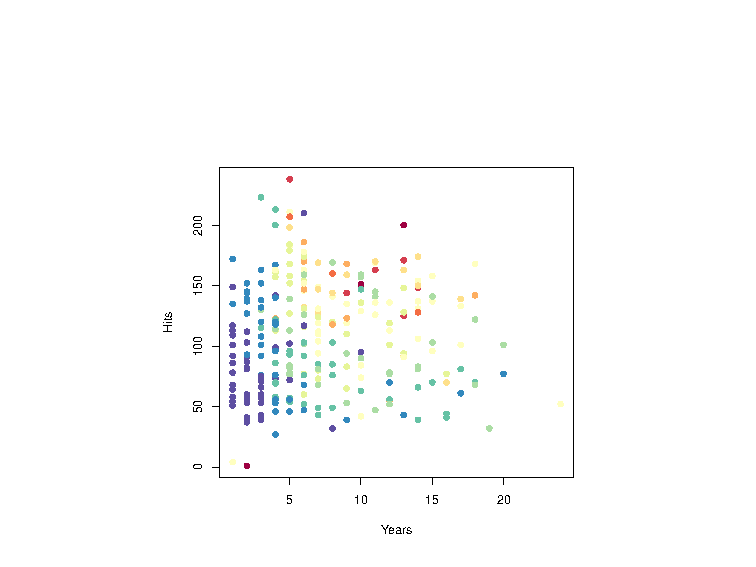
\includegraphics[width=0.55\textwidth]{figures/baseball} \\
    \vspace{-2mm}
    {\tiny Scatter plot of Baseball salary data showing Hits on the y-axis vs Years on the x-axis, with points color-coded by salary.}
\end{frame}

\begin{frame}{Decision tree for these data}
    \centering
    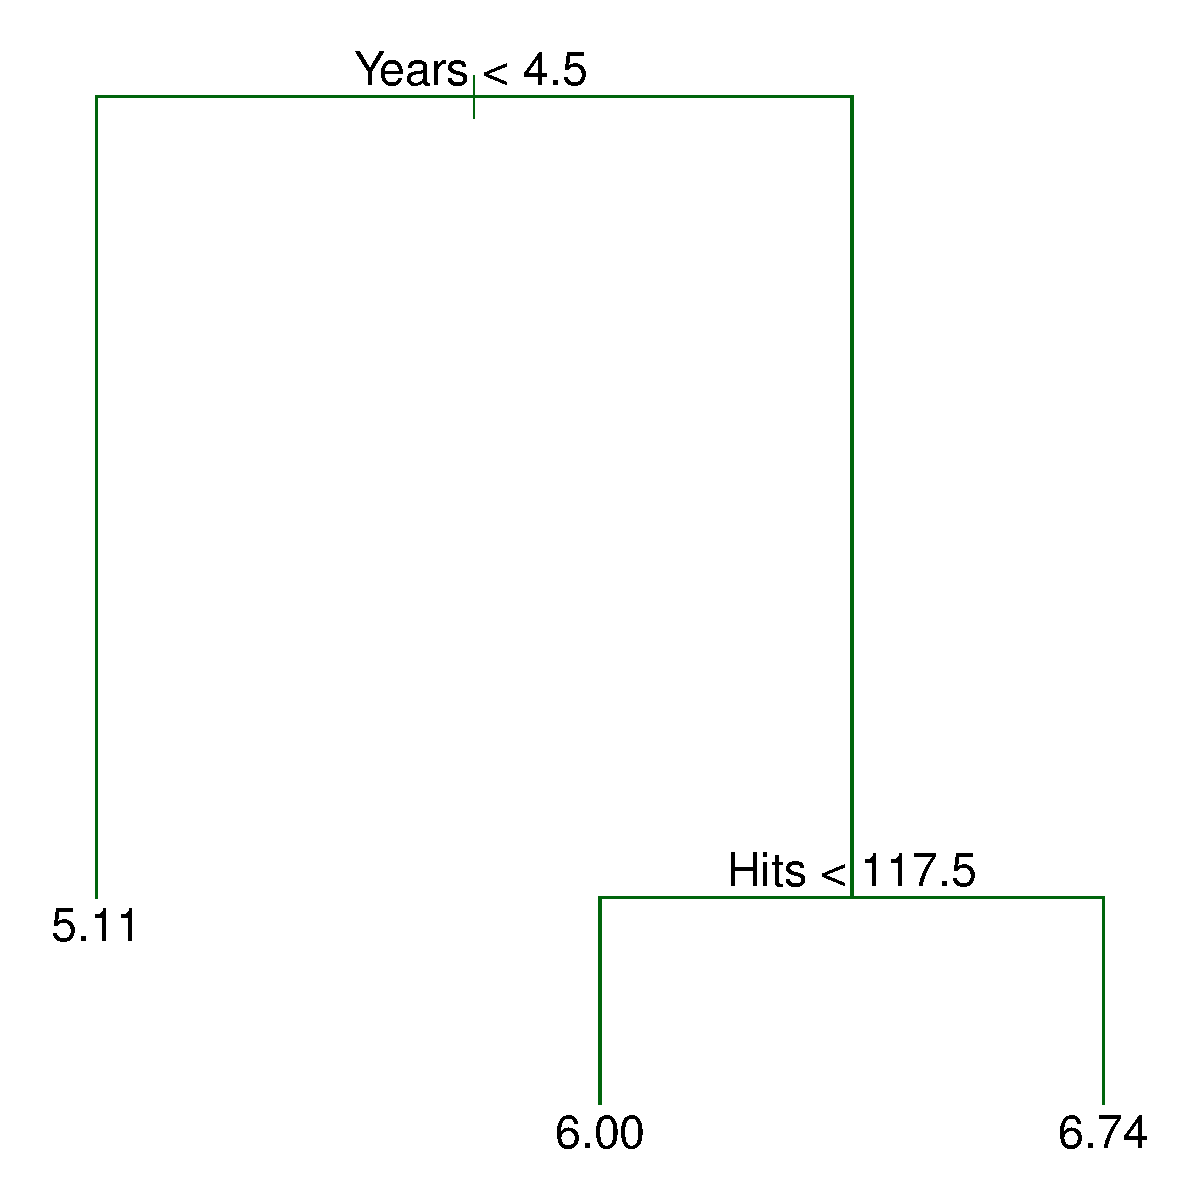
\includegraphics[width=0.45\textwidth]{figures/8_1} \\
    {\tiny A simple regression decision tree for the Baseball salary data. The first split is at $Years < 4.5$. The right branch is further split at $Hits < 117.5$. The terminal leaves show values 5.11, 6.00, and 6.74.}
\end{frame}

\begin{frame}{Details of previous figure}
\begin{itemize}
    \item For the Hitters data, a regression tree for predicting the log salary of a baseball player, based on the number of years that he has played in the major leagues and the number of hits that he made in the previous year.
    \item At a given internal node, the label (of the form $X_{j}<t_{k}$) indicates the left-hand branch emanating from that split, and the right-hand branch corresponds to $X_{j}\ge t_{k}$. For instance, the split at the top of the tree results in two large branches. The left-hand branch corresponds to \texttt{Years} $< 4.5$, and the right-hand branch corresponds to \texttt{Years} $>=4.5$.
    \item The tree has two internal nodes and three terminal nodes, or leaves. The number in each leaf is the mean of the response for the observations that fall there.
\end{itemize}
\end{frame}

\begin{frame}{Results}
    \begin{itemize}
        \item Overall, the tree stratifies or segments the players into three regions of predictor space: $R_{1}=\{X|Years<4.5\}$, $R_{2}=\{X | Years \ge 4.5, Hits<117.5\}$, and $R_{3}=\{X| Years \ge 4.5, Hits \ge 117.5\}$.
    \end{itemize}
    \centering
    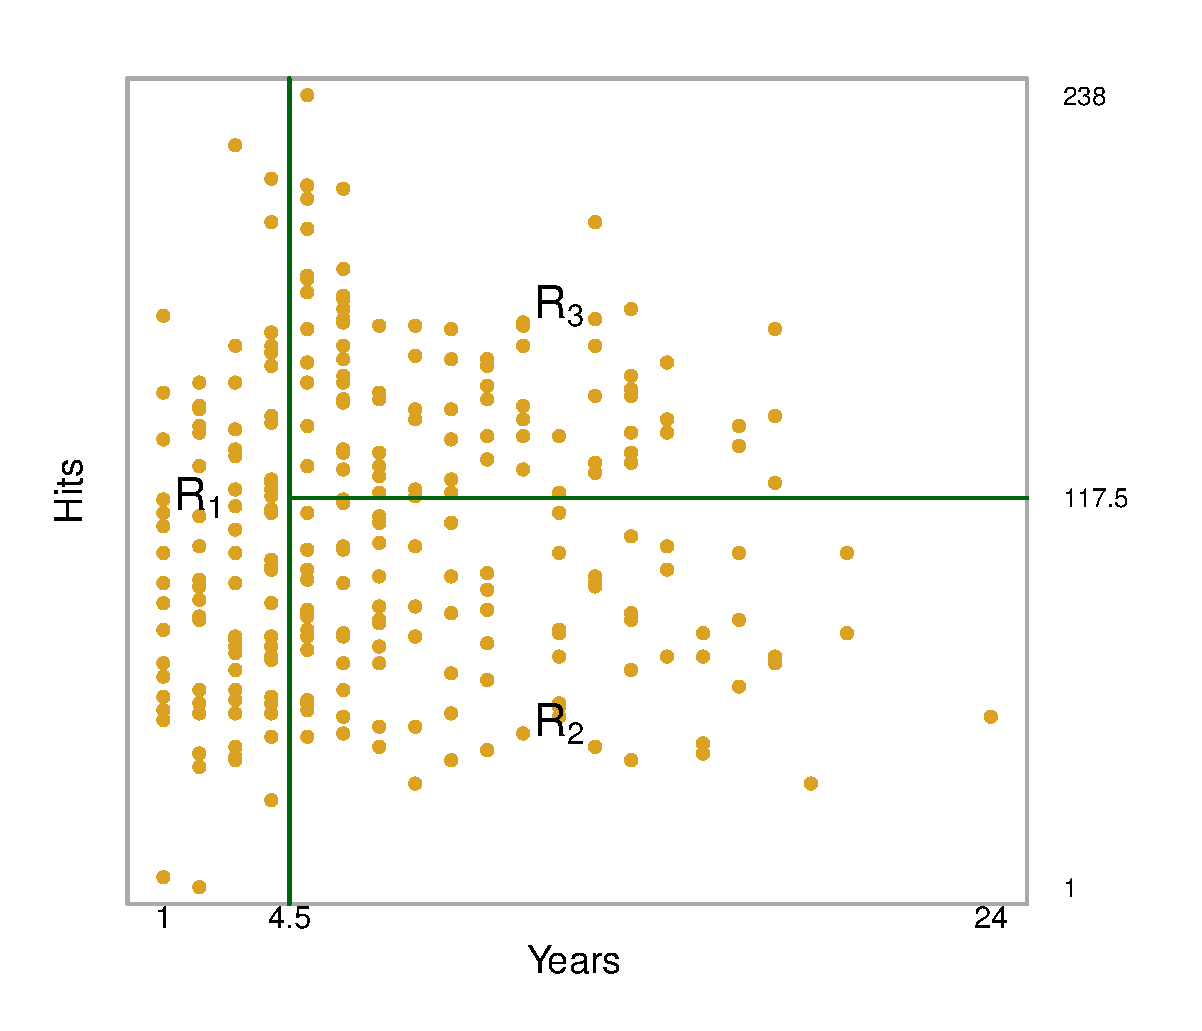
\includegraphics[width=0.4\textwidth]{figures/8_2} \\
    {\tiny Scatter plot of Hits vs Years divided into three rectangular regions ($R_1$, $R_2$, $R_3$) corresponding to the decision tree splits.}
\end{frame}

\begin{frame}{Terminology for Trees}
    \begin{itemize}
        \item In keeping with the \textbf{tree} analogy, the regions $R_{1}$, $R_{2}$, and $R_{3}$ are known as \textbf{terminal nodes}.
        \item Decision trees are typically drawn \textbf{upside down}, in the sense that the leaves are at the bottom of the tree.
        \item The points along the tree where the predictor space is split are referred to as \textbf{internal nodes}.
        \item In the hitters tree, the two internal nodes are indicated by the text \texttt{Years} $< 4.5$ and \texttt{Hits} $< 117.5$.
    \end{itemize}
\end{frame}

\begin{frame}{Interpretation of Results}
    \begin{itemize}
        \item \texttt{Years} is the most important factor in determining \texttt{Salary}, and players with less experience earn lower salaries than more experienced players.
        \item Given that a player is less experienced, the number of \texttt{Hits} that he made in the previous year seems to play little role in his \texttt{Salary}.
        \item But among players who have been in the major leagues for five or more years, the number of \texttt{Hits} made in the previous year does affect \texttt{Salary}, and players who made more \texttt{Hits} last year tend to have higher salaries.
        \item Surely an over-simplification, but compared to a regression model, it is easy to display, interpret and explain.
    \end{itemize}
\end{frame}

\begin{frame}{Details of the tree-building process}
    \begin{enumerate}
        \item We divide the predictor space, that is, the set of possible values for $X_1, X_2, \dots, X_p$, into $J$ distinct and non-overlapping regions, $R_{1},R_{2},...,R_{J}$.
        \item For every observation that falls into the region $R_{j}$, we make the same prediction, which is simply the mean of the response values for the training observations in $R_{j}$.
    \end{enumerate}
\end{frame}

\begin{frame}{More details of the tree-building process}
    \begin{itemize}
        \item In theory, the regions could have any shape. However, we choose to divide the predictor space into high-dimensional rectangles, or \textbf{boxes}, for simplicity and for ease of interpretation of the resulting predictive model.
        \item The goal is to find boxes $R_{1},...,R_{J}$ that minimize the RSS, given by
        \begin{equation*}
        \sum_{j=1}^{J}\sum_{i\in R_{j}}(y_{i}-\hat{y}_{R_{j}})^{2},
        \end{equation*}
        where $\hat{y}_{R_{j}}$ is the mean response for the training observations within the $j_{th}$ box.
    \end{itemize}
\end{frame}

\begin{frame}{More details of the tree-building process}
    \begin{itemize}
        \item Unfortunately, it is computationally infeasible to consider every possible partition of the feature space into $J$ boxes.
        \item For this reason, we take a \textbf{top-down}, \textbf{greedy} approach that is known as recursive binary splitting.
        \item The approach is \textbf{top-down} because it begins at the top of the tree and then successively splits the predictor space; each split is indicated via two new branches further down on the tree.
        \item It is \textbf{greedy} because at each step of the tree-building process, the \textbf{best} split is made at that particular step, rather than looking ahead and picking a split that will lead to a better tree in some future step.
    \end{itemize}
\end{frame}

\begin{frame}{Details Continued}
    \begin{itemize}
        \item We first select the predictor $X_{j}$ and the cutpoint $s$ such that splitting the predictor space into the regions $\{X|X_{j}<s\}$ and $\{X|X_{j}\ge s\}$ leads to the greatest possible reduction in RSS.
        \item Next, we repeat the process, looking for the best predictor and best cutpoint in order to split the data further so as to minimize the RSS within each of the resulting regions.
        \item However, this time, instead of splitting the entire predictor space, we split one of the two previously identified regions. We now have three regions.
        \item Again, we look to split one of these three regions further, so as to minimize the RSS. The process continues until a stopping criterion is reached; for instance, we may continue until no region contains more than five observations.
    \end{itemize}
\end{frame}

\begin{frame}{Predictions}
    \begin{itemize}
        \item We predict the response for a given test observation using the mean of the training observations in the region to which that test observation belongs.
        \item A five-region example of this approach is shown in the next slide.
    \end{itemize}
\end{frame}

\begin{frame}{Partitioning example}
    \centering
    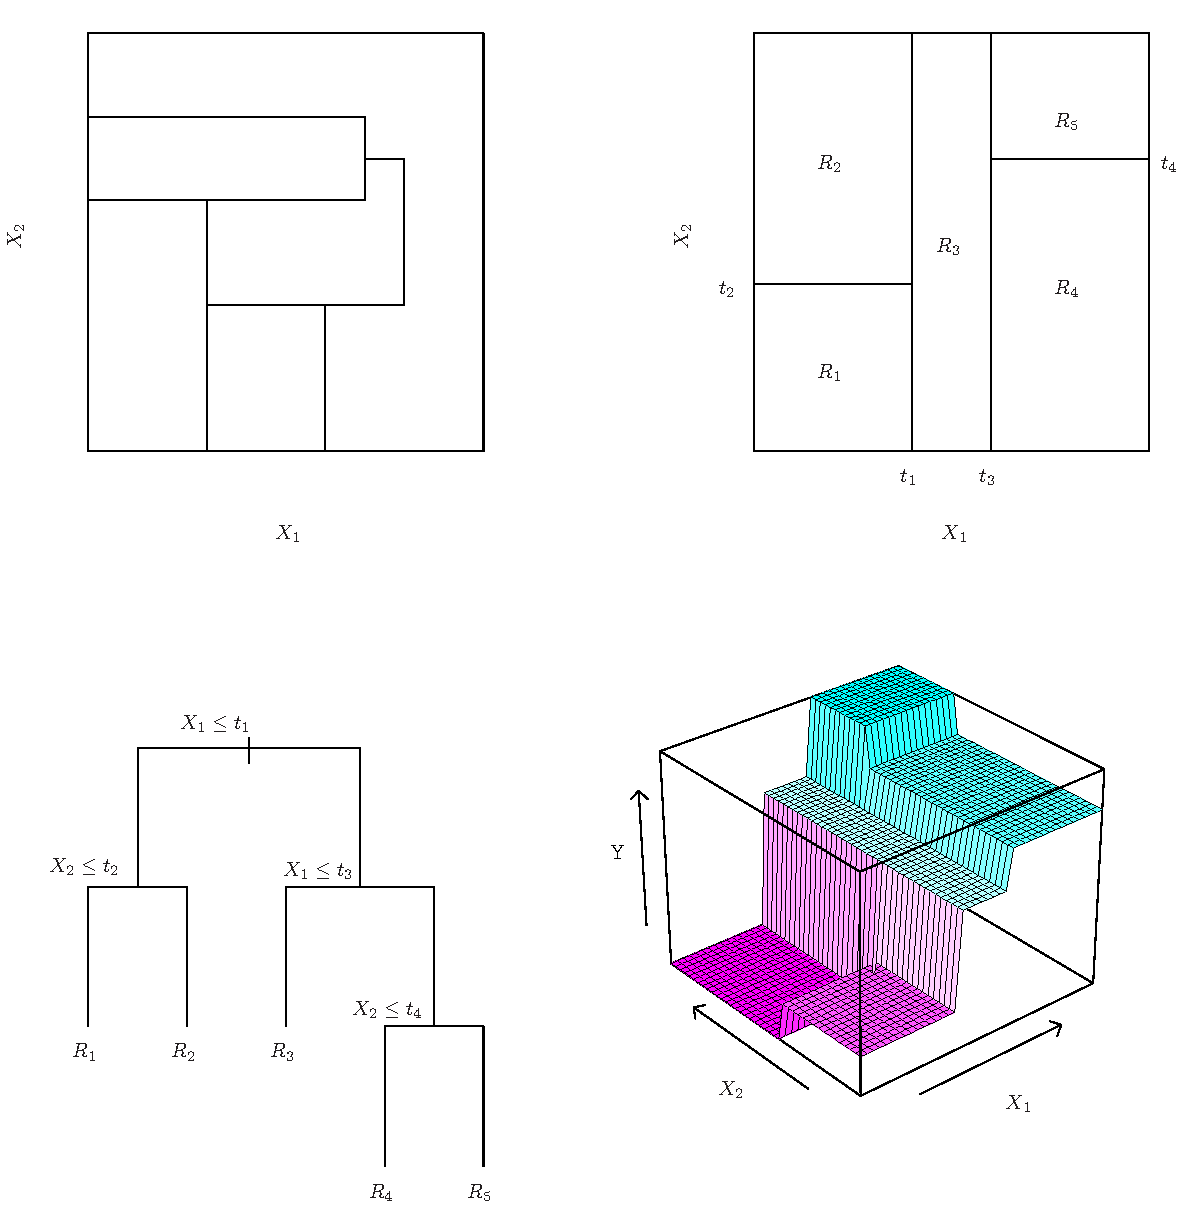
\includegraphics[height=0.9\textheight]{figures/8_3}

    % {\tiny Four panels illustrating recursive binary splitting: Top Left: An invalid partition of two-dimensional feature space. Top Right: Valid output of recursive binary splitting into five regions ($R_1$ to $R_5$). Bottom Left: The corresponding decision tree for the valid partition. Bottom Right: A perspective plot of the prediction surface.}
\end{frame}

\begin{frame}{Details of previous figure}
    \begin{itemize}
        \item Top Left: A partition of two-dimensional feature space that could not result from recursive binary splitting.
        \item Top Right: The output of recursive binary splitting on a two-dimensional example.
        \item Bottom Left: A tree corresponding to the partition in the top right panel.
        \item Bottom Right: A perspective plot of the prediction surface corresponding to that tree.
    \end{itemize}
\end{frame}

\begin{frame}{Pruning a tree}
    \begin{itemize}
        \item The process described above may produce good predictions on the training set, but is likely to \textbf{overfit} the data, leading to poor test set performance. \textbf{Why?} \pause
        \item A smaller tree with fewer splits (that is, fewer regions $R_{1},...,R_{J}$) might lead to lower variance and better interpretation at the cost of a little bias.
        \item One possible alternative to the process described above is to grow the tree only so long as the decrease in the RSS due to each split exceeds some (high) threshold.
        \item This strategy will result in smaller trees, but is too \textbf{short-sighted}: a seemingly worthless split early on in the tree might be followed by a very good split - that is, a split that leads to a large reduction in RSS later on.
    \end{itemize}
\end{frame}

\begin{frame}{Pruning a tree --continued}
    \begin{itemize}
        \item A better strategy is to grow a very large tree $T_{0}$, and then \textbf{prune} it back in order to obtain a \textbf{subtree}.
        \item \textbf{Cost complexity pruning} --also known as \textbf{weakest link pruning}-- is used to do this.
        \item We consider a sequence of trees indexed by a nonnegative tuning parameter $\alpha$. For each value of $\alpha$ there corresponds a subtree $T \subset T_{0}$ such that
        \begin{equation*}
        \sum_{m=1}^{|T|}\sum_{i:x_{i}\in R_{m}}(y_{i}-\hat{y}_{Rm})^{2}+\alpha|T|
        \end{equation*}
        is as small as possible. Here $|T|$ indicates the number of terminal nodes of the tree $T$, $R_{m}$ is the rectangle (i.e. the subset of predictor space) corresponding to the $m_{th}$ terminal node, and $\hat{y}_{R_{m}}$ is the mean of the training observations in $R_{m}$.
    \end{itemize}
\end{frame}

\begin{frame}{Choosing the best subtree}
    \begin{itemize}
        \item The tuning parameter $\alpha$ controls a trade-off between the subtree's complexity and its fit to the training data.
        \item We select an optimal value $\hat{\alpha}$ using cross-validation.
        \item We then return to the full data set and obtain the subtree corresponding to $\hat{\alpha}$.
    \end{itemize}
\end{frame}

\begin{frame}{Summary: tree algorithm}
    \begin{enumerate}
        \item Use recursive binary splitting to grow a large tree on the training data, stopping only when each terminal node has fewer than some minimum number of observations.
        \item Apply cost complexity pruning to the large tree in order to obtain a sequence of best subtrees, as a function of $\alpha$.
        \item Use K-fold cross-validation to choose $\alpha$. For each $k=1,...,K$:
        \begin{itemize}
            \item[3.1] Repeat Steps 1 and 2 on the $\frac{K-1}{K}$th fraction of the training data, excluding the kth fold.
            \item[3.2] Evaluate the mean squared prediction error on the data in the left-out kth fold, as a function of $\alpha$.
        \end{itemize}
        Average the results, and pick $\alpha$ to minimize the average error.
        \item Return the subtree from Step 2 that corresponds to the chosen value of $\alpha$.
    \end{enumerate}
\end{frame}


\begin{frame}{Baseball example continued}
    \begin{itemize}
        \item First, we randomly divided the data set in half, yielding 132 observations in the training set and 131 observations in the test set.
        \item We then built a large regression tree on the training data and varied $\alpha$ in order to create subtrees with different numbers of terminal nodes.
        \item Finally, we performed six-fold cross-validation in order to estimate the cross-validated MSE of the trees as a function of $\alpha$.
    \end{itemize}
\end{frame}

\begin{frame}{Baseball example continued}
    \centering
    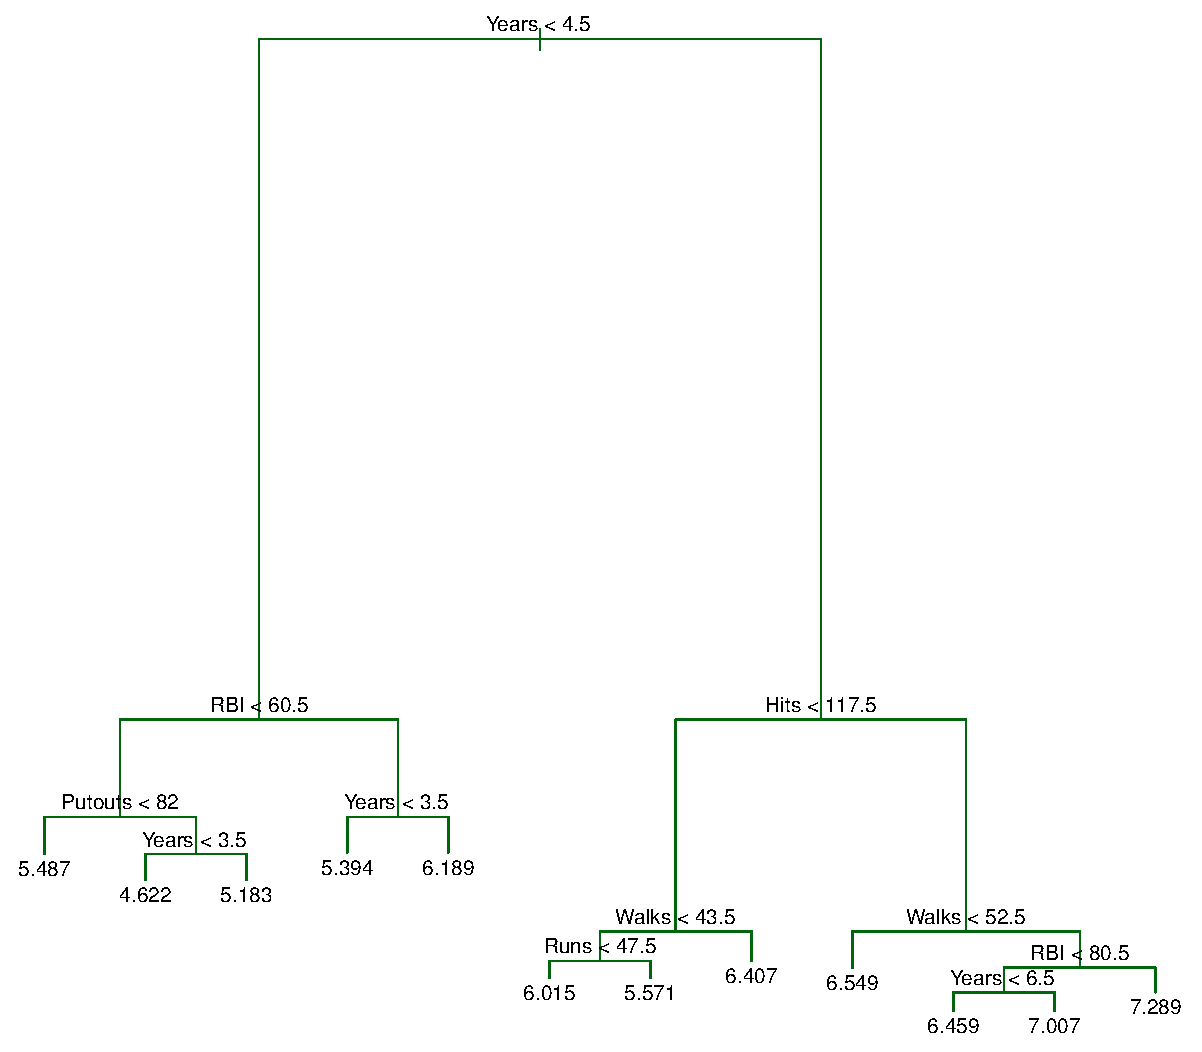
\includegraphics[width=0.6\textwidth]{figures/8_4} \\
    \vspace{-3mm}
    {\tiny A large unpruned regression tree for the Baseball data showing many complex splits.}
\end{frame}

\begin{frame}{Baseball example continued}
    \centering
    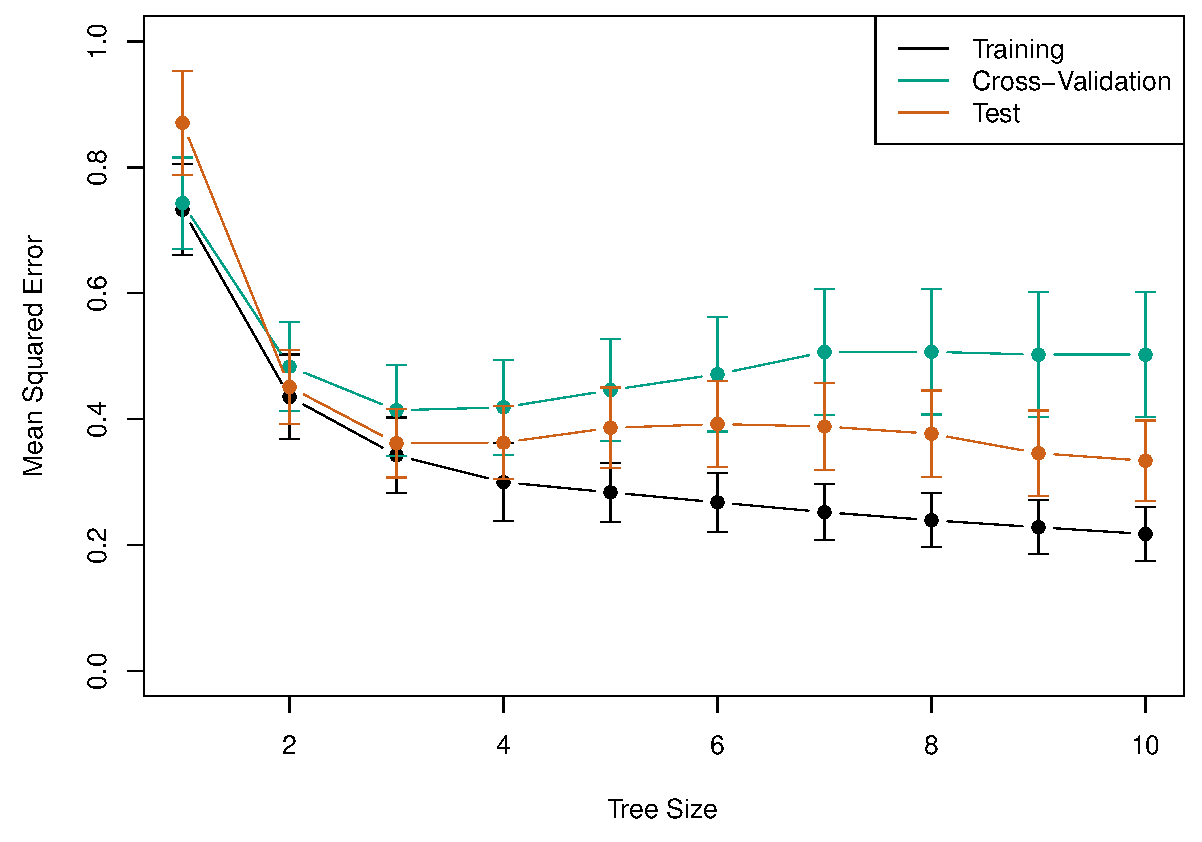
\includegraphics[width=0.7\textwidth]{figures/8_5} \\
    \vspace{-3mm}
    {\tiny Plot of Mean Squared Error versus Tree Size. Three lines are shown: Training Error (decreasing monotonically), Cross-Validation Error (U-shaped, minimum around tree size 3), and Test Error.}
\end{frame}

\begin{frame}{Classification Trees}
    \begin{itemize}
        \item Very similar to a regression tree, except that it is used to predict a qualitative response rather than a quantitative one.
        \item For a classification tree, we predict that each observation belongs to the \textbf{most commonly occurring class} of training observations in the region to which it belongs.
    \end{itemize}
\end{frame}

\begin{frame}{Details of classification trees}
    \begin{itemize}
        \item Just as in the regression setting, we use recursive binary splitting to grow a classification tree.
        \item In the classification setting, RSS cannot be used as a criterion for making the binary splits.
        \item A natural alternative to RSS is the \textbf{classification error rate}. This is simply the fraction of the training observations in that region that do not belong to the most common class:
        \begin{equation*}
        E=1-\max_{k}(\hat{p}_{mk}).
        \end{equation*}
        Here $\hat{p}_{mk}$ represents the proportion of training observations in the $m_{th}$ region that are from the $k_{th}$ class.
        \item However classification error is not sufficiently sensitive for tree-growing, and in practice two other measures are preferable.
    \end{itemize}
\end{frame}

\begin{frame}{Gini index and Deviance}
    \begin{itemize}
        \item The Gini index is defined by
        \begin{equation*}
        G=\sum_{k=1}^{K}\hat{p}_{mk}(1-\hat{p}_{mk}),
        \end{equation*}
        a measure of total variance across the K classes. The Gini index takes on a small value if all of the $\hat{p}_{mk}$ are close to zero or one.
        \item For this reason the Gini index is referred to as a measure of node purity - a small value indicates that a node contains predominantly observations from a single class. \pause
        \item An alternative to the Gini index is cross-entropy, given by
        \begin{equation*}
        D=-\sum_{k=1}^{K}\hat{p}_{mk}\log\hat{p}_{mk}.
        \end{equation*}
        \item It turns out that the Gini index and the cross-entropy are very similar numerically.
    \end{itemize}
\end{frame}

\begin{frame}{Example: heart data}
    \begin{itemize}
        \item These data contain a binary outcome \texttt{HD} for 303 patients who presented with chest pain.
        \item An outcome value of \texttt{Yes} indicates the presence of heart disease based on an angiographic test, while \texttt{No} means no heart disease.
        \item There are 13 predictors including \texttt{Age}, \texttt{Sex}, \texttt{Chol} (a cholesterol measurement), and other heart and lung function measurements.
        \item Cross-validation yields a tree with six terminal nodes. See next figure.
    \end{itemize}
\end{frame}

\begin{frame}{Example: heart data}
    \centering
    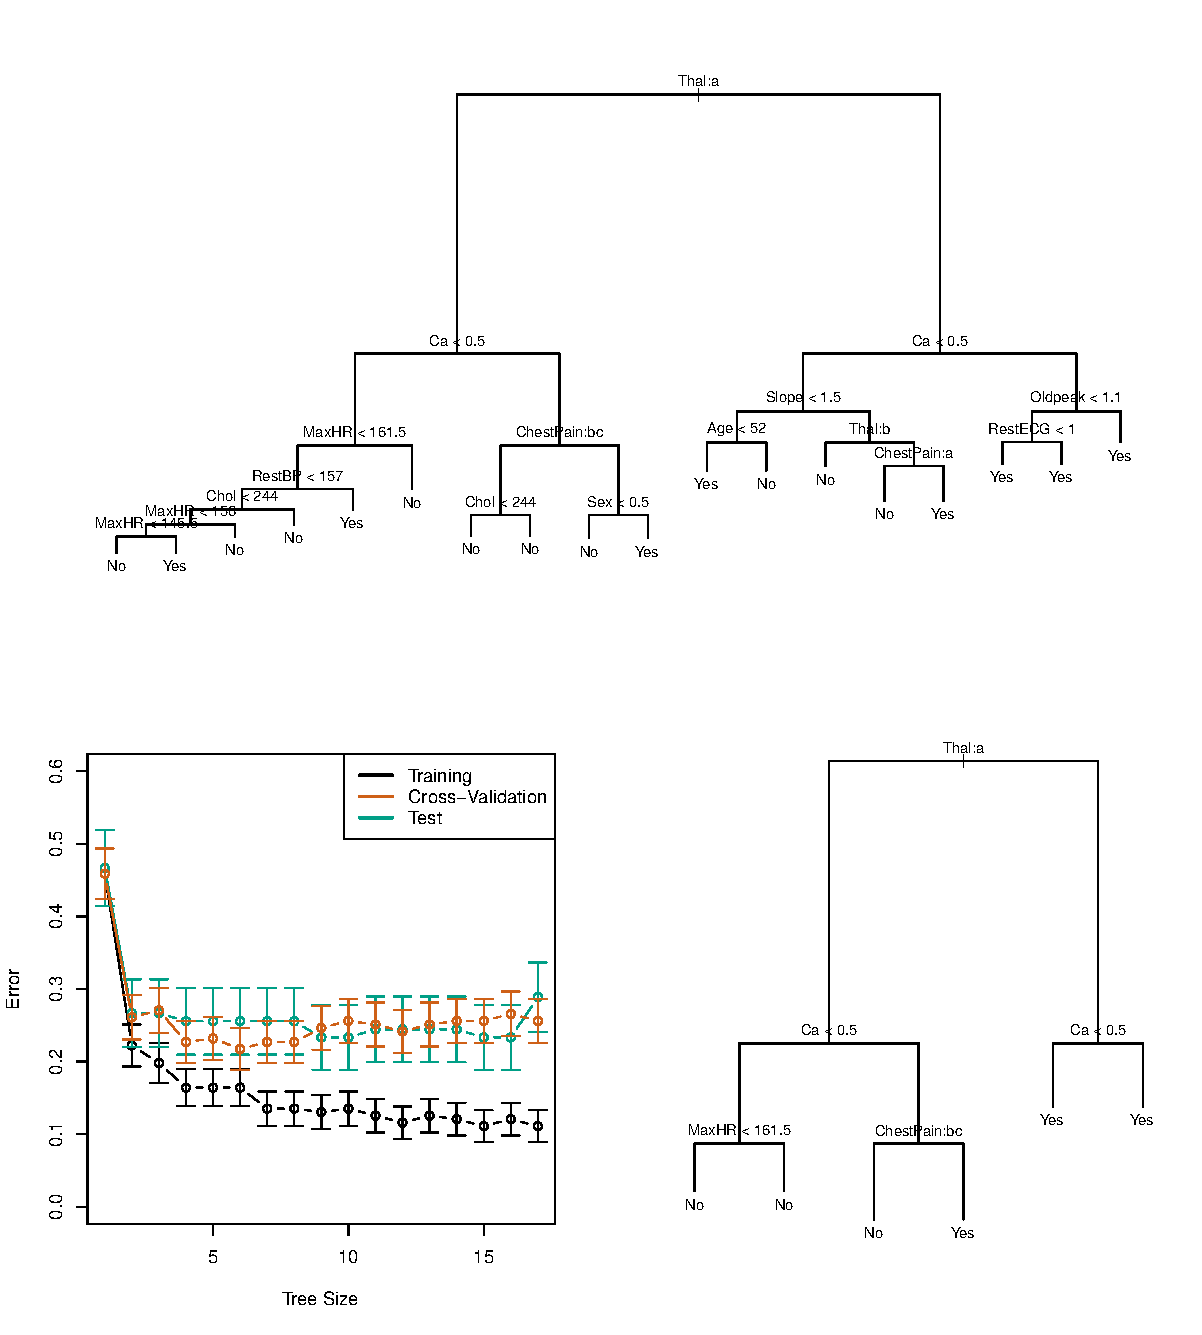
\includegraphics[height=0.9\textheight]{figures/8_6} \\
    % {\tiny Three panels: Top shows an unpruned classification tree for the heart data. Bottom Left shows classification error versus tree size for Training, Cross-Validation, and Test sets. Bottom Right shows the pruned tree with six terminal nodes.}
\end{frame}

\begin{frame}{Trees Versus Linear Models}
    \begin{columns}[c]
        \begin{column}{0.49\textwidth}
            \centering
            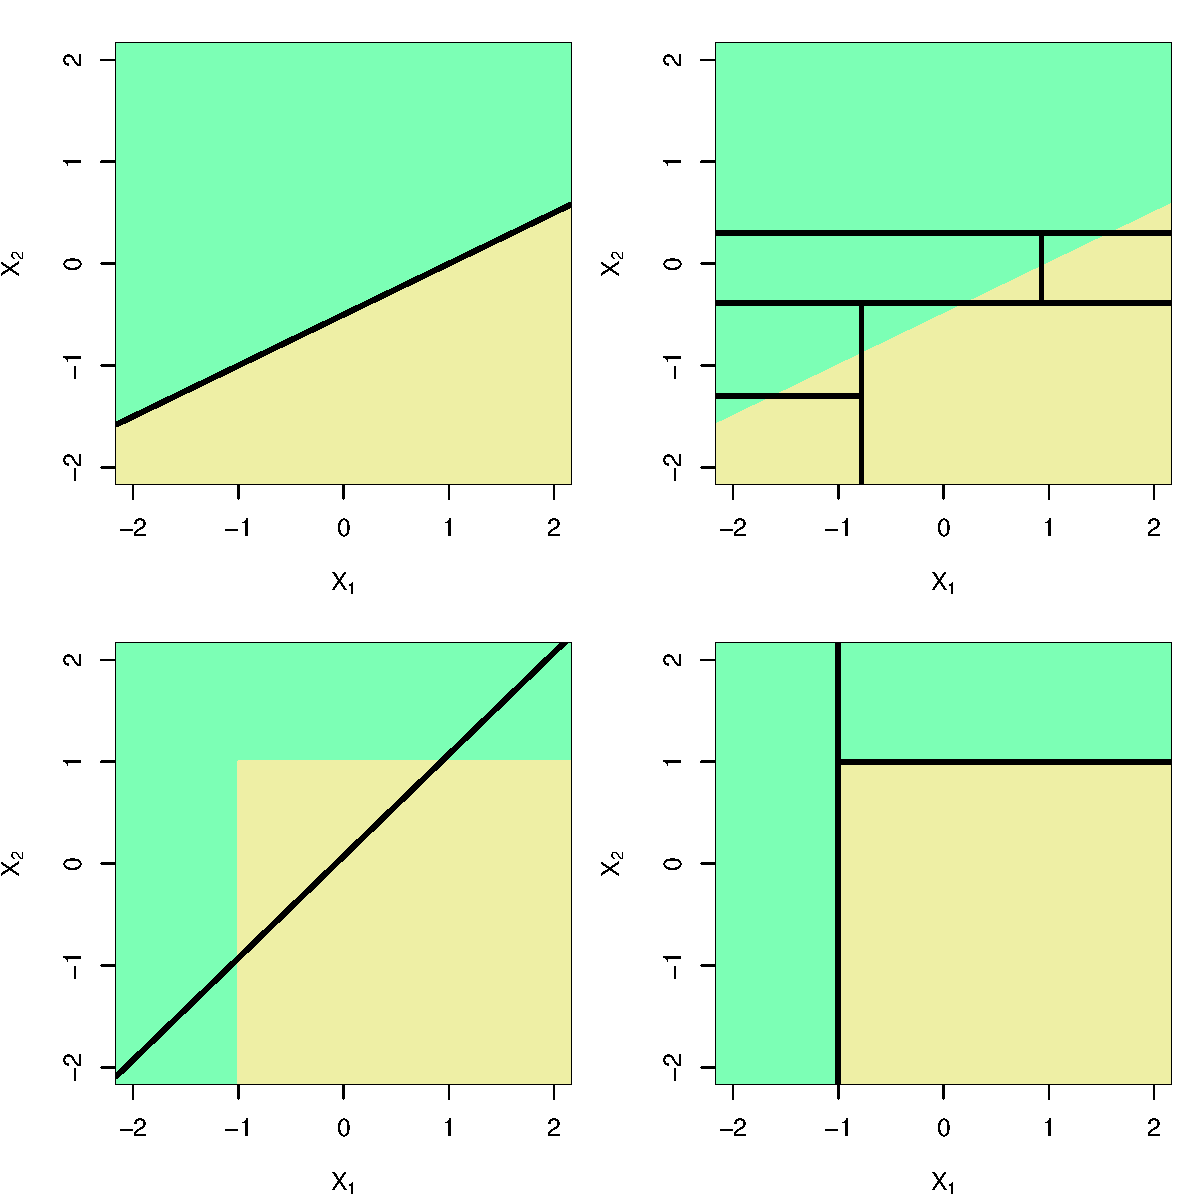
\includegraphics[height=0.8\textheight]{figures/8_7} \\
        \end{column}
        \begin{column}{0.49\textwidth}
            {\scriptsize
            Four panels illustrating boundaries:
                \begin{itemize}
                    \item Top Row shows a true linear boundary;
                    \item Bottom row shows a true non-linear boundary;
                    \item Left column demonstrates a linear model's fit;
                    \item Right column demonstrates a tree-based model's fit.
                \end{itemize}
            Trees handle step-like non-linear boundaries well, while linear models handle diagonal linear boundaries perfectly.
            }
        \end{column}
    \end{columns}
\end{frame}

\begin{frame}{Advantages and Disadvantages of Trees}
    \begin{itemize}
        \item Trees are very easy to explain to people. In fact, they are even easier to explain than linear regression!
        \item Some people believe that decision trees more closely mirror human decision-making than do the regression and classification approaches seen in previous chapters.
        \item Trees can be displayed graphically, and are easily interpreted even by a non-expert (especially if they are small).
        \item Trees can easily handle qualitative predictors without the need to create dummy variables.
        \item Unfortunately, trees generally do not have the same level of predictive accuracy as some of the other regression and classification approaches seen in this book.
    \end{itemize}
    However, by aggregating many decision trees, the predictive performance of trees can be substantially improved. We introduce these concepts next.
\end{frame}

\begin{frame}{Bagging}
    \begin{itemize}
        \item \textbf{Bootstrap aggregation}, or \textbf{bagging}, is a general-purpose procedure for reducing the variance of a statistical learning method; we introduce it here because it is particularly useful and frequently used in the context of decision trees.
        \item Recall that given a set of n independent observations $Z_{1},...,Z_{n}$, each with variance $\sigma^{2}$, the variance of the mean $\overline{Z}$ of the observations is given by $\sigma^{2}/n$.
        \item In other words, \textbf{averaging a set of observations reduces variance}. Of course, this is not practical because we generally do not have access to multiple training sets.
    \end{itemize}
\end{frame}

\begin{frame}{Bagging --continued}
    \begin{itemize}
        \item Instead, we can bootstrap, by taking repeated samples from the (single) training data set.
        \item In this approach we generate $B$ different bootstrapped training data sets. We then train our method on the $b_{th}$ bootstrapped training set in order to get $\hat{f}^{*b}(x)$, the prediction at a point x. We then average all the predictions to obtain
        \begin{equation*}
        \hat{f}_{bag}(x)=\frac{1}{B}\sum_{b=1}^{B}\hat{f}^{*b}(x).
        \end{equation*}
        This is called \textbf{bagging}.
    \end{itemize}
\end{frame}

\begin{frame}{Bagging classification trees}
    \begin{itemize}
        \item The above prescription applied to regression trees.
        \item For classification trees: for each test observation, we record the class predicted by each of the $B$ trees, and take a \textbf{majority vote}: the overall prediction is the most commonly occurring class among the $B$ predictions.
    \end{itemize}
\end{frame}

\begin{frame}{Bagging the heart data}
    \centering
    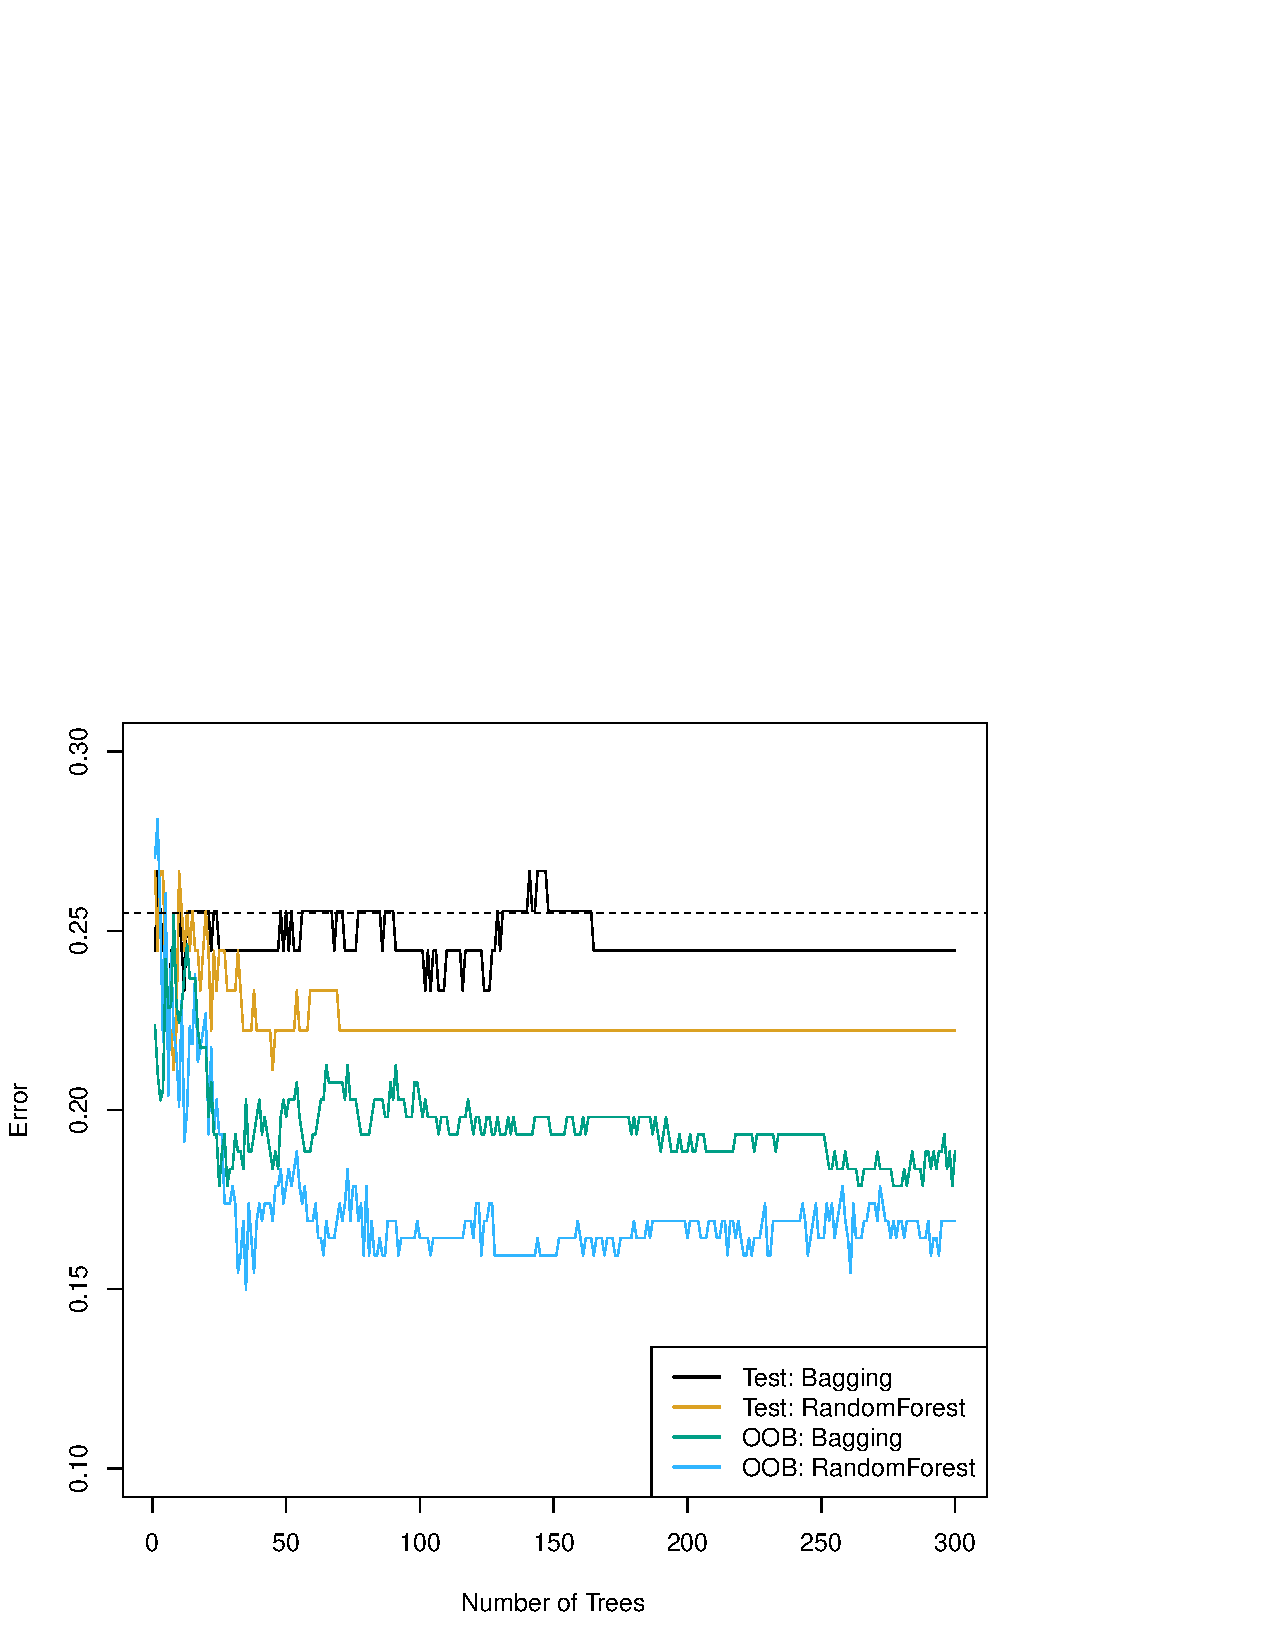
\includegraphics[height=0.8\textheight]{figures/8_8} \\
    \vspace{-3mm}
    {\tiny Plot of Error vs Number of Trees for the Heart data. It compares Test error and Out-Of-Bag (OOB) error for both Bagging and Random Forests. Random forest error stabilizes lower than bagging error.}
\end{frame}

\begin{frame}{Details of previous figure}
    Bagging and random forest results for the Heart data.
    \begin{itemize}
        \item The test error (black and orange) is shown as a function of $B$, the number of bootstrapped training sets used.
        \item Random forests were applied with $m=\sqrt{p}$.
        \item The dashed line indicates the test error resulting from a single classification tree.
        \item The green and blue traces show the OOB error, which in this case is considerably lower.
    \end{itemize}
\end{frame}

\begin{frame}{Out-of-Bag Error Estimation}
\begin{itemize}
    \item It turns out that there is a very straightforward way to estimate the test error of a bagged model.
    \item Recall that the key to bagging is that trees are repeatedly fit to bootstrapped subsets of the observations. One can show that on average, each bagged tree makes use of around two-thirds of the observations.
    \item The remaining one-third of the observations not used to fit a given bagged tree are referred to as the \textbf{out-of-bag} (OOB) observations.
    \item We can predict the response for the ith observation using each of the trees in which that observation was OOB. This will yield around $B/3$ predictions for the ith observation, which we average.
    \item This estimate is essentially the LOO\footnote{Leave-One-Out} cross-validation error for bagging, if $B$ is large.
\end{itemize}
\end{frame}

\begin{frame}{Random Forests}
    \begin{itemize}
        \item \textbf{Random forests} provide an improvement over bagged trees by way of a small tweak that \textbf{decorrelates} the trees. This reduces the variance when we average the trees.
        \item As in bagging, we build a number of decision trees on bootstrapped training samples.
        \item But when building these decision trees, each time a split in a tree is considered, \textbf{a random selection of $m$ predictors} is chosen as split candidates from the full set of $p$ predictors. The split is allowed to use only one of those $m$ predictors.
        \item A fresh selection of $m$ predictors is taken at each split, and typically we choose $m \approx \sqrt{p}$ that is, the number of predictors considered at each split is approximately equal to the square root of the total number of predictors (4 out of the 13 for the \texttt{Heart} data).
    \end{itemize}
\end{frame}

\begin{frame}{Example: gene expression data}
    \begin{itemize}
        \item We applied random forests to a high-dimensional biological data set consisting of expression measurements of 4,718 genes measured on tissue samples from 349 patients.
        \item There are around 20,000 genes in humans, and individual genes have different levels of activity, or expression, in particular cells, tissues, and biological conditions.
        \item Each of the patient samples has a qualitative label with 15 different levels: either normal or one of 14 different types of cancer.
        \item We use random forests to predict cancer type based on the 500 genes that have the largest variance in the training set.
        \item We randomly divided the observations into a training and a test set, and applied random forests to the training set for three different values of the number of splitting variables $m$.
    \end{itemize}
\end{frame}

\begin{frame}{Results: gene expression data}
    \centering
    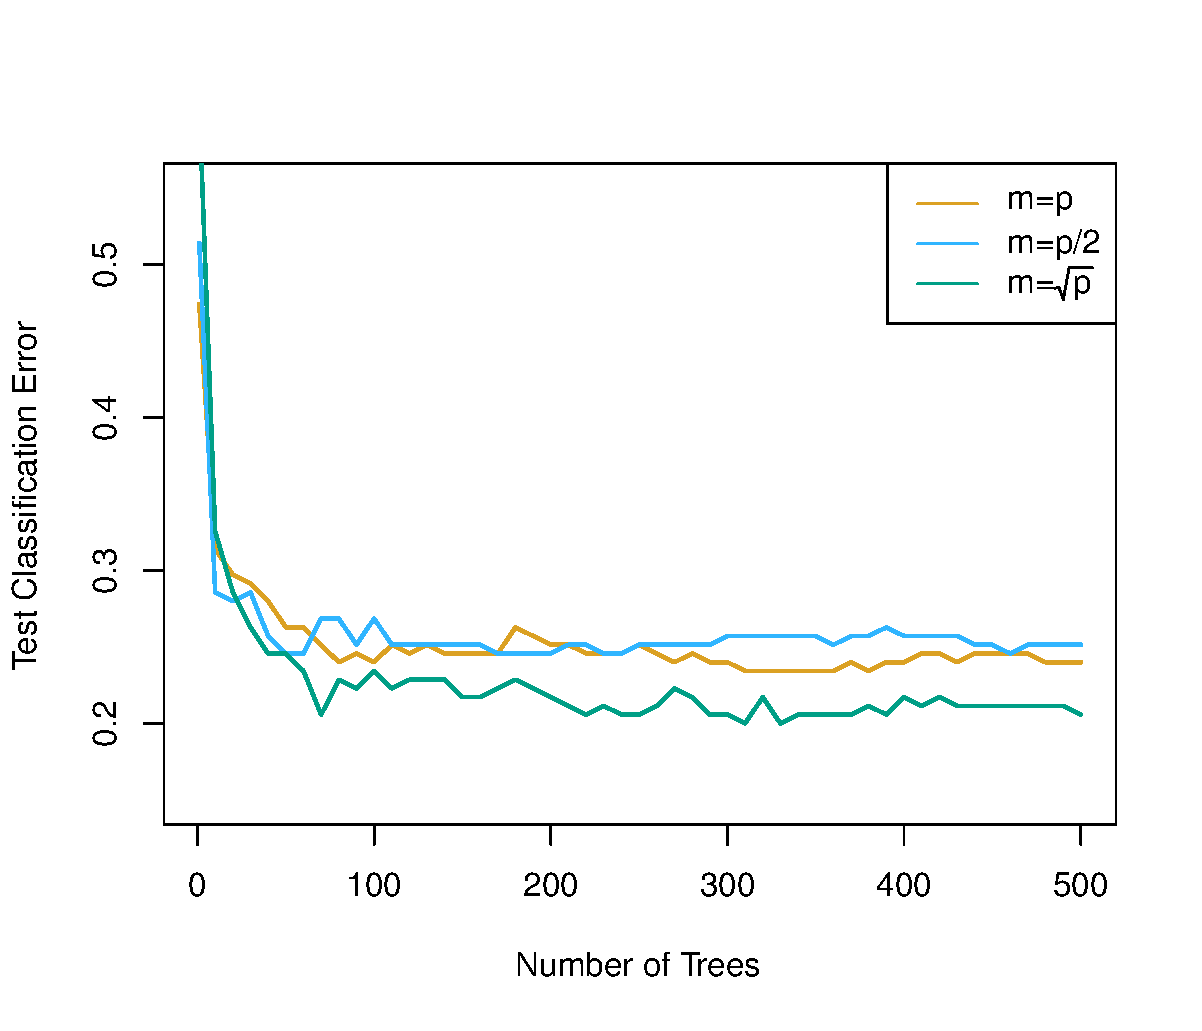
\includegraphics[width=0.8\textwidth]{figures/8_10} \\
    \vspace{-3mm}
    % {\tiny Plot of Test Classification Error vs Number of Trees for gene expression data. It compares results using $m=p$, $m=p/2$, and $m=\sqrt{p}$. Lower values of $m$ (Random Forests) yield lower test error than $m=p$ (Bagging).}
\end{frame}

\begin{frame}{Details of previous figure}
\begin{itemize}
    \item Results from random forests for the fifteen-class gene expression data set with $p=500$ predictors.
    \item The test error is displayed as a function of the number of trees. Each colored line corresponds to a different value of m, the number of predictors available for splitting at each interior tree node.
    \item Random forests ($m<p$) lead to a slight improvement over bagging ($m=p$). A single classification tree has an error rate of 45.7\%.
\end{itemize}
\end{frame}

\begin{frame}{Boosting}
    \begin{itemize}
        \item Like bagging, boosting is a general approach that can be applied to many statistical learning methods for regression or classification. We only discuss boosting for decision trees.
        \item Recall that bagging involves creating multiple copies of the original training data set using the bootstrap, fitting a separate decision tree to each copy, and then combining all of the trees in order to create a single predictive model.
        \item Notably, each tree is built on a bootstrap data set, independent of the other trees.
        \item Boosting works in a similar way, except that the trees are grown \textbf{sequentially}: each tree is grown using information from previously grown trees.
    \end{itemize}
\end{frame}

\begin{frame}{Boosting algorithm for regression trees}
\begin{enumerate}
    \item Set $\hat{f}(x)=0$ and $r_{i}=y_{i}$ for all i in the training set.
    \item For $b=1,2,...,B$, repeat:
    \begin{itemize}
        \item[2.1] Fit a tree $\hat{f}^{b}$ with $d$ splits ($d+1$ terminal nodes) to the training data $(X, r)$.
        \item[2.2] Update $\hat{f}$ by adding in a shrunken version of the new tree: $$\hat{f}(x)\leftarrow\hat{f}(x)+\lambda\hat{f}^{b}(x)$$.
        \item[2.3] Update the residuals, $$r_{i}\leftarrow r_{i}-\lambda\hat{f}^{b}(x_{i})$$.
    \end{itemize}
    \item Output the boosted model,
    \begin{equation*}
    \hat{f}(x)=\sum_{b=1}^{B}\lambda\hat{f}^{b}(x).
    \end{equation*}
\end{enumerate}
\end{frame}

\begin{frame}{What is the idea behind this procedure?}
\begin{itemize}
    \item Unlike fitting a single large decision tree to the data, which amounts to \textbf{fitting the data hard} and potentially overfitting, the boosting approach instead \textbf{learns slowly}.
    \item Given the current model, we fit a decision tree to the residuals from the model. We then add this new decision tree into the fitted function in order to update the residuals.
    \item Each of these trees can be rather small, with just a few terminal nodes, determined by the parameter d in the algorithm.
    \item By fitting small trees to the residuals, we slowly improve $\hat{f}$ in areas where it does not perform well. The shrinkage parameter $\lambda$ slows the process down even further, allowing more and different shaped trees to attack the residuals.
\end{itemize}
\end{frame}

\begin{frame}{Boosting for classification}
\begin{itemize}
    \item Boosting for classification is similar in spirit to boosting for regression, but is a bit more complex. We will not go into detail here, nor do we in the text book.
    \item Students can learn about the details in \textbf{Elements of Statistical Learning, chapter 10}.
    \item The \texttt{R} package \texttt{gbm} (gradient boosted models) handles a variety of regression and classification problems.
\end{itemize}
\end{frame}

\begin{frame}{Gene expression data continued}
    \centering
    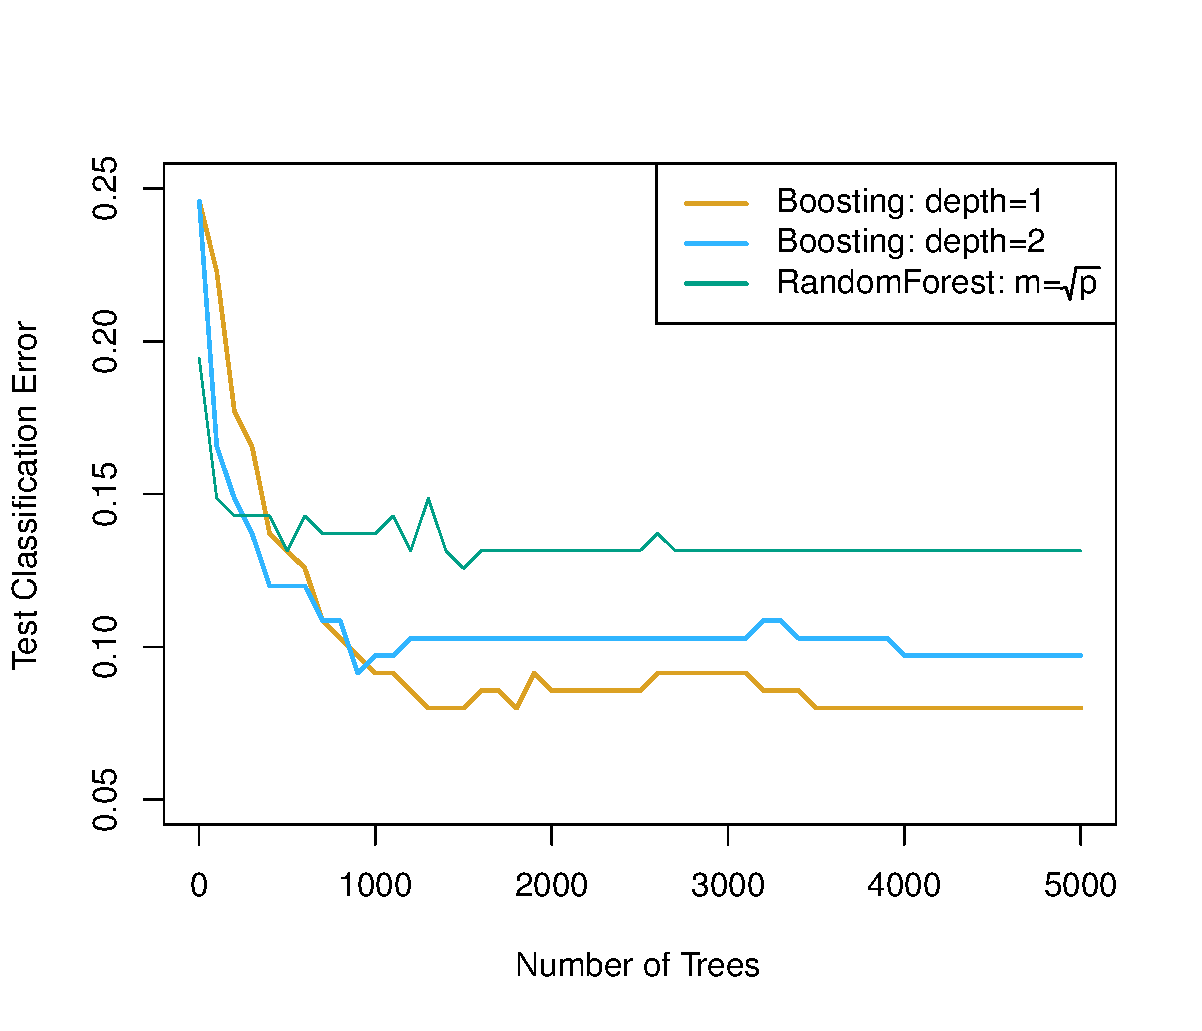
\includegraphics[width=0.75\textwidth]{figures/8_11}
    % {\tiny Plot of Test Classification Error vs Number of Trees for the gene expression data. It compares Boosting with depth=1, Boosting with depth=2, and Random Forest ($m=\sqrt{p}$). Both boosting models outperform the random forest model.}
\end{frame}

\begin{frame}{Details of previous figure}
\begin{itemize}
    \item Results from performing boosting and random forests on the fifteen-class gene expression data set in order to predict \textbf{cancer} versus \textbf{normal}.
    \item The test error is displayed as a function of the number of trees. For the two boosted models, $\lambda=0.01$. Depth-1 trees slightly outperform depth-2 trees, and both outperform the random forest, although the standard errors are around 0.02, making none of these differences significant.
    \item The test error rate for a single tree is 24\%.
\end{itemize}
\end{frame}

\begin{frame}{Tuning parameters for boosting}
\begin{enumerate}
    \item The \textbf{number of trees} $B$. Unlike bagging and random forests, boosting can overfit if B is too large, although this overfitting tends to occur slowly if at all. We use cross-validation to select B. \pause
    \item The \textbf{shrinkage parameter} $\lambda$, a small positive number. This controls the rate at which boosting learns. Typical values are 0.01 or 0.001, and the right choice can depend on the problem. Very small $\lambda$ can require using a very large value of B in order to achieve good performance. \pause
    \item The \textbf{number of splits} $d$ in each tree, which controls the complexity of the boosted ensemble. Often $d=1$ works well, in which case each tree is a \textbf{stump}, consisting of a single split and resulting in an additive model. More generally $d$ is the \textbf{interaction depth}, and controls the interaction order of the boosted model, since $d$ splits can involve at most d variables.
\end{enumerate}
\end{frame}

\begin{frame}{Another regression example}
    \centering
    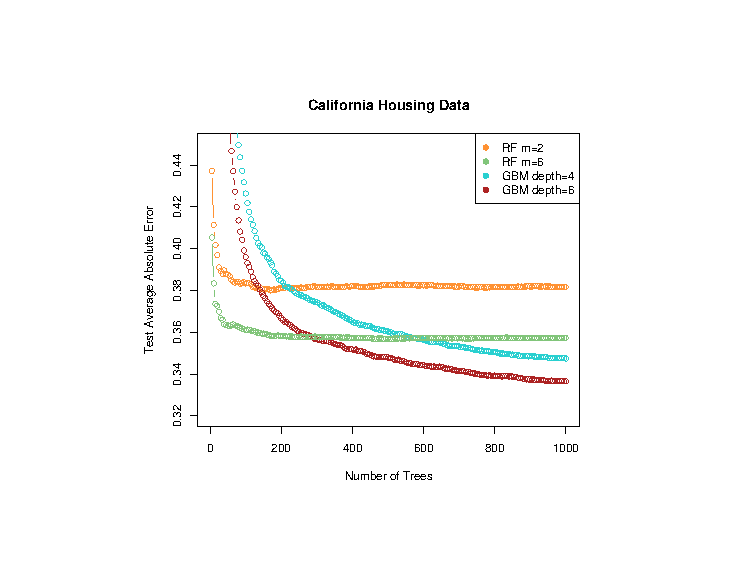
\includegraphics[width=0.6\textwidth]{figures/housing} \\
    \vspace{-2mm}
    {\tiny Boosting achieves lower error faster as trees are added.}
\end{frame}

\begin{frame}{Another classification example}
    \centering
    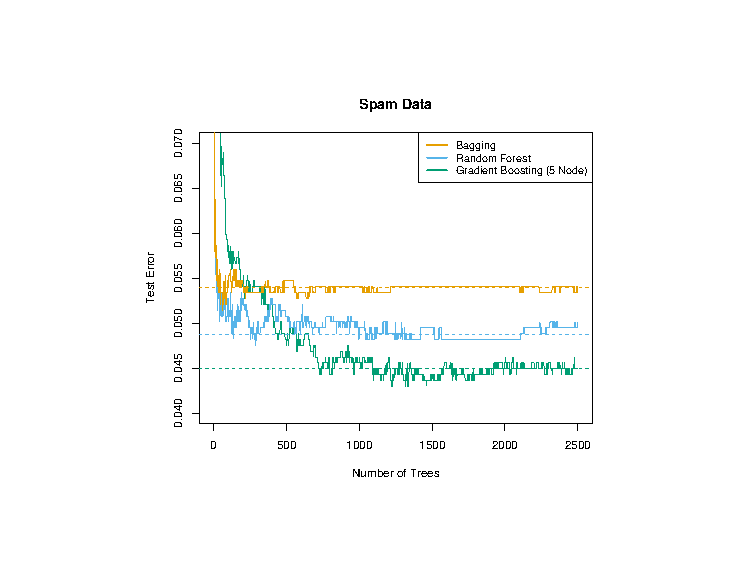
\includegraphics[width=0.6\textwidth]{figures/spam} \\
    \vspace{-2mm}
    {\tiny Gradient Boosting eventually achieves the lowest test error.}
\end{frame}

\begin{frame}{Variable importance measure}
    \begin{itemize}
        \footnotesize
        \item For bagged/RF regression trees, we record the total amount that the RSS is decreased due to splits over a given predictor, averaged over all $B$ trees. A large value indicates an important predictor.
        \item Similarly, for bagged/RF classification trees, we add up the total amount that the Gini index is decreased by splits over a given predictor, averaged over all $B$ trees.
    \end{itemize}
    \begin{columns}[c]
        \begin{column}{0.39\textwidth}
            \centering
            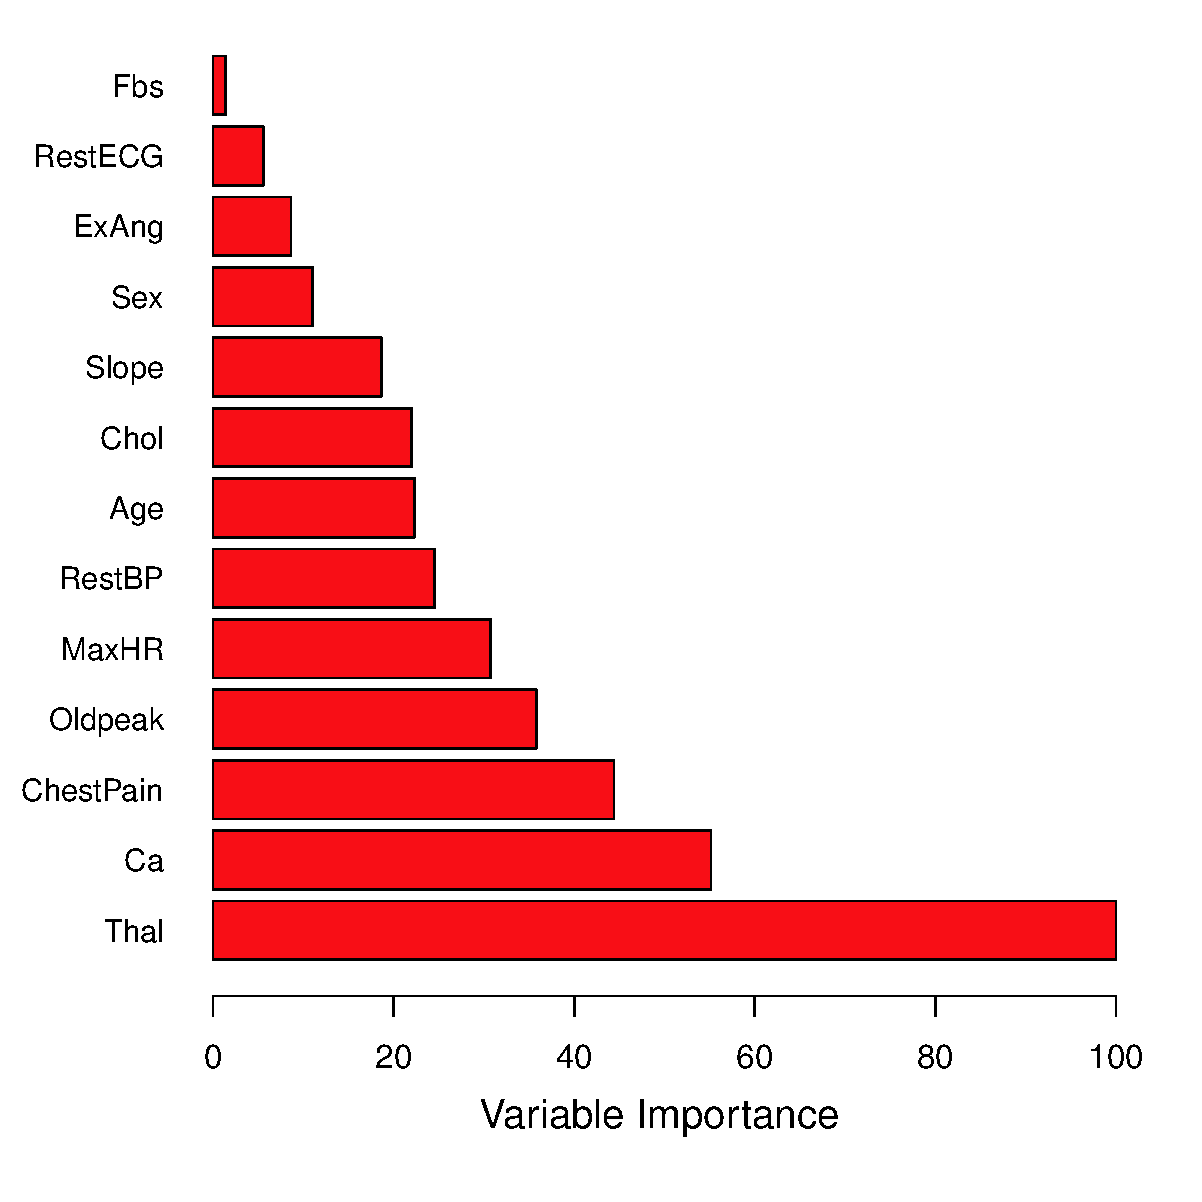
\includegraphics[width=\textwidth]{figures/8_9}
        \end{column}
        \begin{column}{0.59\textwidth}
            \footnotesize
            Horizontal bar chart showing \textit{Variable Importance} for the \texttt{Heart} data. \texttt{Thal}, \texttt{Ca}, and \texttt{ChestPain} are the top three most important variables.
        \end{column}
    \end{columns}

\end{frame}

\begin{frame}{Summary}
    \begin{itemize}
        \item Decision trees are simple and interpretable models for regression and classification.
        \item However they are often not competitive with other methods in terms of prediction accuracy.
        \item Bagging, random forests and boosting are good methods for improving the prediction accuracy of trees. They work by growing many trees on the training data and then combining the predictions of the resulting ensemble of trees.
        \item The latter two methods, random forests and boosting, are among the state-of-the-art methods for supervised learning. However their results can be difficult to interpret.
    \end{itemize}
\end{frame}

\begin{frame}{}
    \centering
    \Huge End of Chapter 8.
\end{frame}

\begin{frame}{An Introduction to Statistical Learning with Applications in R}{a.k.a. ISLR}
    \centering
    
\includegraphics[height=0.7\textheight]{figures/book_cover} \\
    \vspace{4mm}
    {
        \tiny
        Content has been extracted from \textit{An Introduction to Statistical Learning with Applications in R}, Second Edition, by James, Witten, Hastie \& Tibshirani. Springer. 2023.\\
        Visit \url{https://www.statlearning.com/}.\\
    }
\end{frame}

\end{document}
